\documentclass{article}
\usepackage{amsfonts, amsmath, amssymb, amsthm, dsfont} % Math notations imported
\usepackage{enumitem}
\usepackage{graphicx}
\usepackage{setspace}
\usepackage{indentfirst}
\usepackage[margin=1in]{geometry}
\graphicspath{{./images/}} % Path to images

% \begin{figure}[htb!]
%      \centering
%      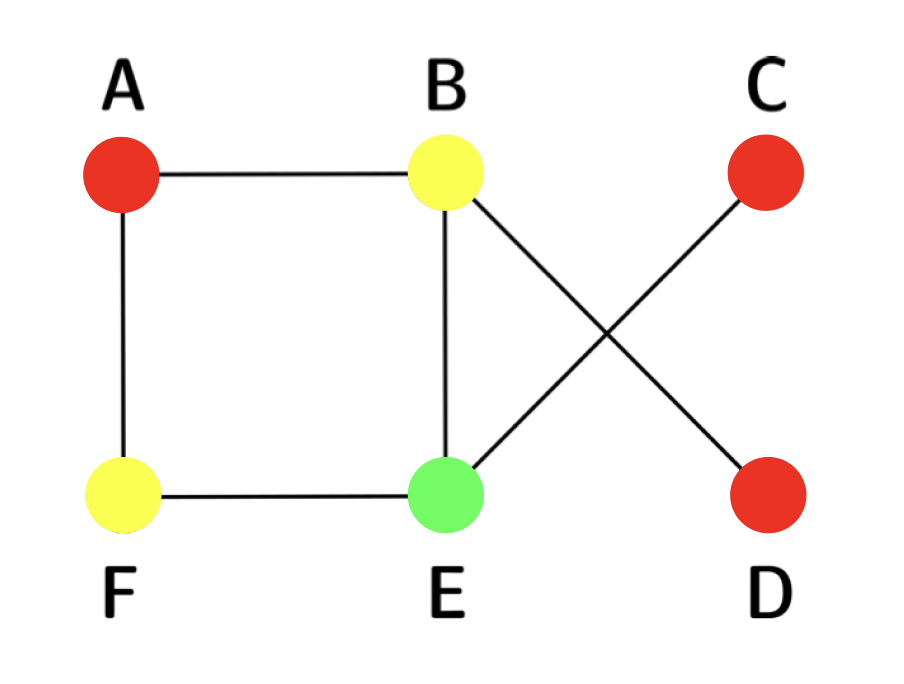
\includegraphics[scale=0.5]{coloring.png}
%      \caption{Coloring of the graph.}
% \end{figure}

% \begin{figure}[htb]
%     \qquad
%     \begin{minipage}{.4\textwidth}
%         \centering
%         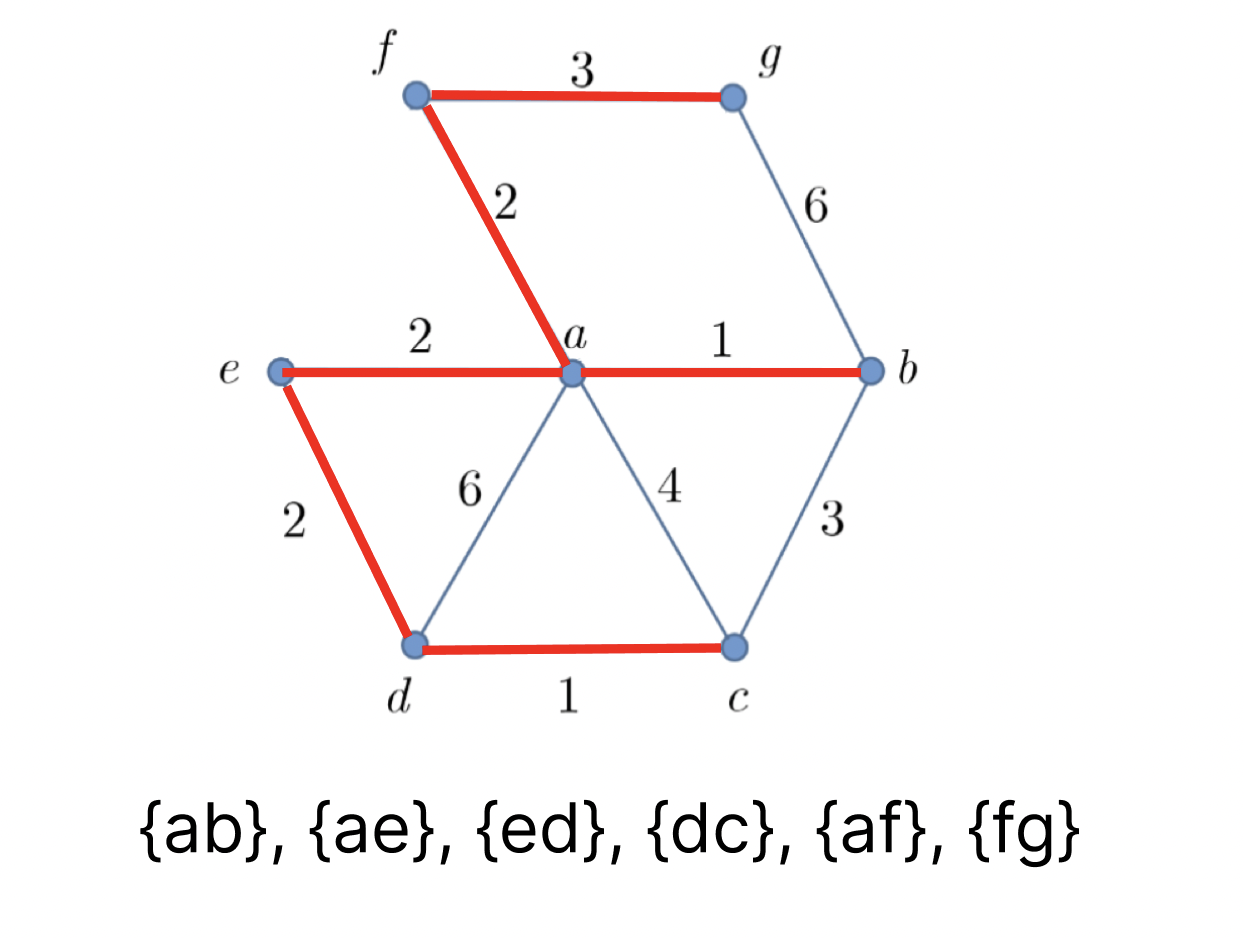
\includegraphics[scale=0.35]{prims.png}
%         \caption{}
%     \end{minipage}    
%     \qquad
%     \begin{minipage}{.4\textwidth}
%         \centering
%         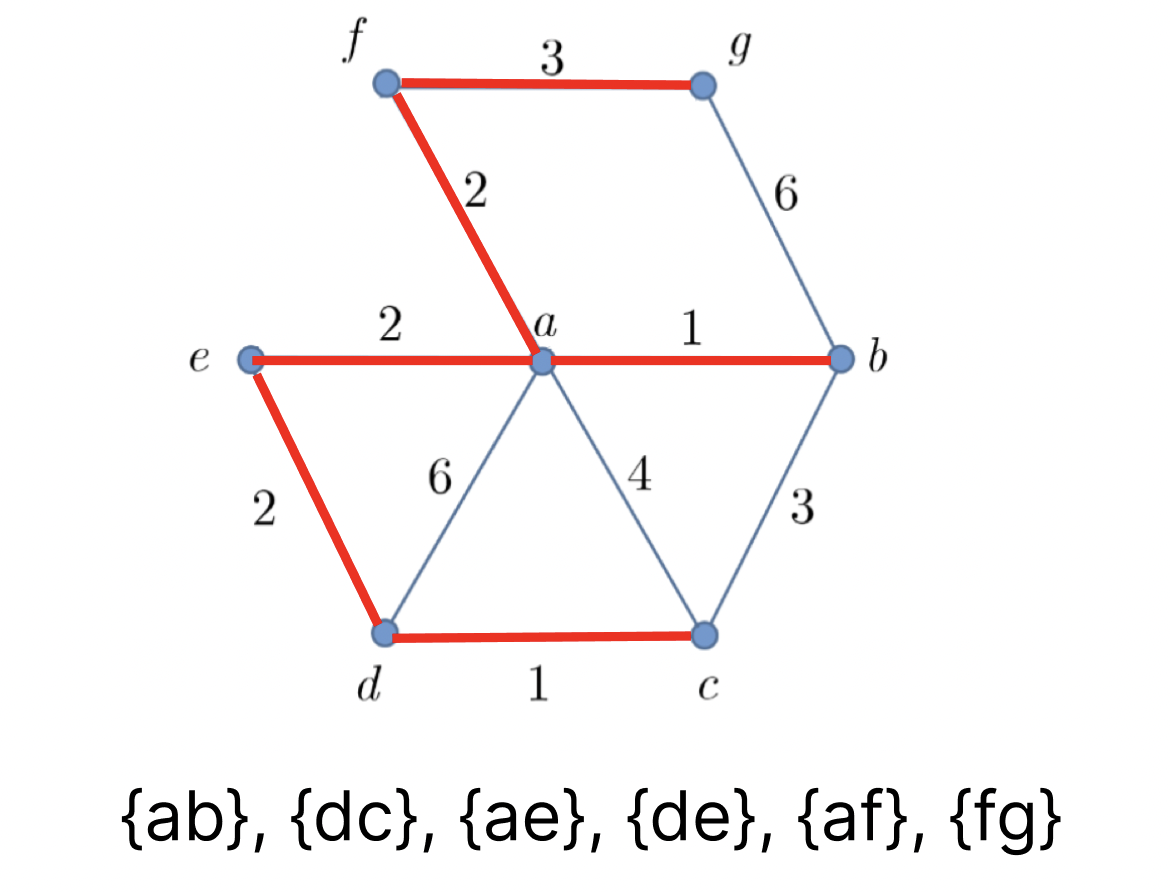
\includegraphics[scale=0.35]{kruskal.png}
%         \caption{}
%     \end{minipage}        
% \end{figure} 

\newtheorem{thm}{Theorem}
\newtheorem{proposition}[thm]{Proposition}
\newtheorem{corollary}[thm]{Corollary}
\newtheorem{lemma}[thm]{Lemma}

\newcommand*{\Var}{\ensuremath{\mathrm{Var}}}
\newcommand*{\Cov}{\ensuremath{\mathrm{Cov}}}
\newcommand*{\Corr}{\ensuremath{\mathrm{Corr}}}
\newcommand*{\Bias}{\ensuremath{\mathrm{Bias}}}
\newcommand*{\MSE}{\ensuremath{\mathrm{MSE}}}
\newcommand*{\range}{\ensuremath{\mathrm{range}}\,}
\newcommand*{\spann}{\ensuremath{\mathrm{span}}\,}
\newcommand*{\nul}{\ensuremath{\mathrm{null}}\,}
\newcommand*{\dom}{\ensuremath{\mathrm{dom}}\,}
\renewcommand*{\implies}{\ensuremath{\Longrightarrow}}
\renewcommand*{\impliedby}{\ensuremath{\Longleftarrow}}
\newcommand*{\Z}{\ensuremath{\mathbb{Z}}}
\newcommand*{\Q}{\ensuremath{\mathbb{Q}}}
\newcommand*{\R}{\ensuremath{\mathbb{R}}}
\newcommand*{\F}{\ensuremath{\mathbb{F}}}
\newcommand*{\C}{\ensuremath{\mathbb{C}}}
\newcommand*{\N}{\ensuremath{\mathbb{N}}}
\newcommand*{\E}{\ensuremath{\mathds{E}}}
\renewcommand*{\P}{\ensuremath{\mathds{P}}}
\newcommand*{\p}{\ensuremath{\mathcal{P}}}

% title information
\title{Math 110 HW8}
\author{Neo Lee}
\date{10/28/2023}

\setstretch{1.15}
% main content
\begin{document} 

% placing title information; comment out if using fancyhdr
\maketitle 

\subsection*{Problem 1.}
Let $p\in {\cal P}(\C)$. Define $q: \C \to \C$ by the formula
$$ q(z):= p(z) \overline{p(\overline{z})}.$$
Prove that $q\in   {\cal P}(\R)$. If $\deg p=n$, then what is $\deg q$? Explain.
\begin{proof}
    Write 
    $$p(z)= a_0 + \cdots + a_nz^n,$$
    then 
    \begin{align*}
        & \overline{p(z)} = \overline{a_0 + \cdots + a_nz^n} = 
        \overline{a_0} + \cdots + \overline{a_nz^n} = \overline{a_0} + \cdots + \overline{a_n}\cdot\overline{z^n} \\
        \implies \quad & \overline{p(\overline{z})} = \overline{a_0} + \cdots + \overline{a_n}\cdot\overline{\overline{z}^n} 
        = \overline{a_0} + \cdots + \overline{a_n}\cdot\overline{\overline{z^n}} 
        = \overline{a_0} + \cdots + \overline{a_n}\cdot z^n 
        = \sum_{k=0}^{n}\overline{a_k}\cdot z^k.
    \end{align*}
    Therefore, our desired result is
    \begin{align*}
        p(z) \overline{p(\overline{z})} &= \left(\sum_{j=0}^{n}a_j\cdot z^j\right)
        \left(\sum_{k=0}^{n}\overline{a_k}\cdot z^k\right) \\
        &= \sum_{k=0}^{n}a_k\cdot \overline{a_k}\cdot z^{2k} + 
        \sum_{j\neq k}a_j\cdot \overline{a_k}\cdot z^{j+k} \\
        & = \sum_{k=0}^{n}|a_k|^2\cdot z^{2k} + \sum_{j>k} (a_j\cdot \overline{a_k}+ 
        \overline{a_j}\cdot a_k)\cdot z^{j+k} \\
        & = \sum_{k=0}^{n}|a_k|^2\cdot z^{2k} + \sum_{j>k} (a_j\cdot \overline{a_k}+ 
        \overline{a_j\cdot \overline{a_k}})\cdot z^{j+k} \\
        & = \sum_{k=0}^{n}|a_k|^2\cdot z^{2k} + \sum_{j>k} \left(2\,\mathrm{Re}\,(a_j\cdot\overline{a_k})\right)\cdot z^{j+k},
    \end{align*}
    where we can see all the coefficients are real numbers.

    If $\deg p = n$, then from the polynomial expression above, we can see the highest 
    degree term is $z^{2n}$, so $\deg q = 2n$.
\end{proof}

\newpage
\subsection*{Problem 2.}
Let $V={\cal P}_3(\R)$ and let $D$ denote the differentiation operator on $V$. 
Determine, with proof,  all subspaces of $V$ invariant under the action of $D$. 
\begin{proof}
    We note that $\p_0(\R), \p_1(\R), \p_2(\R), \p_3(\R)$ are all invariant subspaces because 
    for any vector $p\in \p_k(\R)$, $D$ acting on $p$ will simply reduce the polynomial degree by 1, 
    and hence fall back into $\p_k(\R)$. Also, the zero subspace is invariant because $D(0)=0$.

    We claim that there are no more other invariant subspaces. 
    
    Assume for contradiction that there exists 
    another invariant subspace $W$ with $\dim W = m \le 4$, then we take the polynomial with largest 
    degree in $W$ and call it $p$. Notice $\deg p \ge m-1$, otherwise all the polynomials have 
    degree $\le m-2$ and hence $W$ is a subspace of $\p_{m-2}(\R)$ with $\dim W\le m-1$. At the same time, 
    $\deg p \le m-1$ because otherwise $(p,\dots, D^mp)$ will all be in $W$ and they 
    are linearly independent due to different degrees. Therefore, $\deg p = m-1$ \implies 
    $W$ is a subspace of $\p_{m-1}(\R)$ with the same dimension of $\p_{m-1}(\R)$ \implies 
    $W = \p_{m-1}(\R)$, which is already included in the invariant subspaces we found above. 
\end{proof}

\newpage
\subsection*{Problem 3.}
Suppose $V$ is a finite-dimensional complex vector space and  $T\in {\cal L}(V)$ satisfies the 
condition: For any $\varphi\in V'$ and any $v\in V$, $\lim_{n\to \infty} \varphi(T^n v)=0.$ What 
does this imply about the eigenvalues of $T$? 
\begin{proof}
    We claim that all eigenvalues of $T$ must be less than 1. Consider two contradictory cases: 
    \begin{enumerate}
        \item [(1) $\exists \lambda = 1$:] 
        There exists eigenvector $v\neq 0$ such that $T^nv = \lambda^nv=v$ for $n\in\N$. Then we can
        construct $\phi$ that sends all vectors in $V\setminus \spann(v)$ to 0 while 
        $\phi(cv) = c$ for $c\in\F$. Therefore, $\lim_{n\to\infty}\phi(T^nv)=
        \lim_{n\to\infty}\phi(v)=1\neq 0$, a contradiction.
        
        \item [(2) $\exists \lambda > 1$:] There exists eigenvector $v\neq 0$ such that 
        $T^nv = \lambda^nv$ for $n\in\N$. Again, we construct the same $\phi$. Then 
        $\phi(T^nv)=\phi(\lambda^nv)=\lambda^n$ \implies $\lim_{n\to\infty}\phi(T^nv)=\lim_{n\to\infty}\lambda^n=
        \infty\neq 0$, a contradiction.
    \end{enumerate}
\end{proof}

\newpage
\subsection*{Problem 4.}
Suppose $V$ is finite-dimensional, $T \in {\cal L}(V)$ has $\dim V$ distinct eigenvalues,
and $S \in {\cal L}(V)$ has the same eigenvectors as $T$ (not necessarily with with the same eigenvalues).
\textbf{(a)} Prove that $TS=ST$. \textbf{(b)} Give an example of such operators $T$ and $S$ on $\R^2$, neither of 
which is a multiple of the identity operator.
\begin{proof} Notation: $\dim V=n$.
    \begin{enumerate}[label=(\alph*)]
        \item $T$ has $n$ distinct eigenvalues \implies $T$ has $n$ linearly independent 
        eigenvectors with each eigenvector corresponding to a distinct eigenvalue. Therefore, 
        this set of eigenvectors forms a basis of $V$; denote the set of eigenvectors as
        $\{v_1,\dots,v_n\}$.
        
        Now we evaluate the action of $TS$ and $ST$ on any arbitrary $v\in V$:
        \begin{align*}
            TS(v) & = T(S(a_1v_1 + \cdots + a_nv_n)) \\
            & = T(S(a_1v_1) + \cdots + S(a_nv_n)) \\
            & = T(a_1S(v_1) + \cdots + a_nS(v_n)) \\
            & = T(a_1\gamma_1v_1 + \cdots + a_n\gamma_nv_n) \\
            & = T(a_1\gamma_1v_1) + \cdots + T(a_n\gamma_nv_n) \\
            & = a_1\gamma_1T(v_1) + \cdots + a_n\gamma_nT(v_n) \\
            & = a_1\gamma_1\lambda_1v_1 + \cdots + a_n\gamma_n\lambda_nv_n \\
            & = a_1\lambda_1\gamma_1v_1 + \cdots + a_n\lambda_n\gamma_nv_n \\
            & = a_1\lambda_1S(v_1) + \cdots + a_n\lambda_nS(v_n) \\
            & = S(a_1\lambda_1v_1) + \cdots + S(a_n\lambda_nv_n) \\
            & = S(a_1T(v_1)) + \cdots + S(a_nT(v_n)) \\
            & = S(T(a_1v_1)) + \cdots + S(T(a_nv_n)) \\
            & = S(T(a_1v_1) +\cdots T(a_nv_n)) \\
            & = S(T(a_1v_1+\cdots a_nv_n)) \\
            & = S(T(v)),
        \end{align*}
        where $\gamma_k$ is the corresponding eiganvalues of $S$ for $v_k$ while 
        $\lambda_k$ is the corresponding eigenvalues of $T$ for $v_k$.

        \item Let 
        $$T:(x,y)\mapsto (2x,3y),$$
        then $T$ has eigenvalues 2 and 3 with eigenvectors $(1,0)$ and $(0,1)$ respectively.
        Let $$S:(x,y)\mapsto (5x,10y),$$ then $S$ has eigenvalues 5 and 10 with eigenvectors
        $(1,0)$ and $(0,1)$ respectively. Therefore, 
        $$TS(x,y) = T(5x,10y) = (10x,30y) = 5(2x,3y) = 5T(x,y) = ST(x,y).$$
    \end{enumerate}
\end{proof}


\newpage
\subsection*{Problem 5.}
Let $S, T\in {\cal L}(V)$ and suppose $S$ is invertible. (a) Prove that, for any polynomial 
$p\in {\cal P}({\F})$,  $$ p(STS^{-1}) = S\, p(T) \, S^{-1}.$$  (b) How are the subspaces of $V$ 
invariant under $T$ related to the subspaces invariant under $STS^{-1}$?
\begin{proof}\indent 
    \begin{enumerate}[label=(\alph*)]
        \item
        \textbf{Lemma:} \emph{For any linear map $T$ and invertible linear map $S$, $(STS^{-1})^n = 
        ST^nS^{-1}$.} 
        \begin{proof}
            We show by induction on $\N$.
            
            Base Case: $(STS^{-1})^1 = STS^{-1}$ trivially.

            Inductive Step:
            \begin{align*}
                (STS^{-1})^{k+1} & = (STS^{-1})^k(STS^{-1}) \\
                & = (ST^kS^{-1})(STS^{-1}) \qquad (\emph{applying inductive hypothesis})\\
                & = ST^k(S^{-1}S)TS^{-1} \\
                & = ST^kTS^{-1} \\
                & = ST^{k+1}S^{-1}.
            \end{align*}

            Hence, the lemme is shown by mathematical induction.
        \end{proof}


        Write $$p(STS^{-1}) = a_0I + a_1STS^{-1} + \cdots + a_n(STS^{-1})^n,$$ then 
        for $v\in V$,
        \begin{align*}
            p(STS^{-1})(v) & = (a_0I + a_1STS^{-1} + \cdots + a_n(STS^{-1})^n)(v) \\
            & = a_0I(v) + a_1STS^{-1}(v) + \cdots + a_n(STS^{-1})^n(v) \\
            & = a_0I(v) + a_1STS^{-1}(v) + \cdots + a_nST^nS^{-1}(v) \\
            & = a_0SS^{-1}(v) + a_1STS^{-1}(v) + \cdots + a_nST^nS^{-1}(v) \\
            & = Sa_0S^{-1}(v) + Sa_1TS^{-1}(v) + \cdots + Sa_nT^nS^{-1}(v) \\
            & = S(a_0TS^{-1}(v) + a_1TS^{-1}(v) + \cdots + a_nT^nS^{-1}(v)) \\
            & = S(a_0T + a_1T + \cdots + a_nT^n)\left(S^{-1}(v)\right) \\
            & = S(p(T))S^{-1}(v) \\
        \end{align*}

        \item 
        If $W$ is an invariant subspace of $T$, then $S(W)$ is an invariant subapsce of 
        $STS^{-1}$ because for any vector $v\in S(W)$, $S^{-1}$ first maps the vector to $W$ and applying $T$ will map back into 
        $W$, and eventually applying $S$ will map it back to $S(W)$.
    \end{enumerate}
\end{proof}

\end{document}
